\subsection{Short introduction to nuclear and particle physics}
In order to understand the notions of half life period and nuclear fission we need to
give a short introduction into nuclear and particle physics, herefore we follow \cite{Hooshyar}.
Let now in the following be $Z$ - atomic number,  $N$ - number of neutrons and  $A$ - the number of nuclei, also
called nucleon number, such that $A = Z + N$. The electric charge of the nucleus in ground state is $+Z e$.
It is common now to describe the so called nuclides with $_{Z}^{A}\textrm{Y}$.\\
The Forces that bind the nuclei in the nuclei contribute to the total mass of an atom in terms of the 
binding energy $\Delta E = \Delta M c^2$:
\begin{equation}
\Delta M = M_{tot.} - Z(M_p + M_e) - N M_n
\end{equation}
Where we used the proton, electron and neutron masses $M_p$, $M_e$ and $M_n$ 
(see figure~/ref{fig:bindingenergy}).
\begin{figure}[htpb]
    \centering
    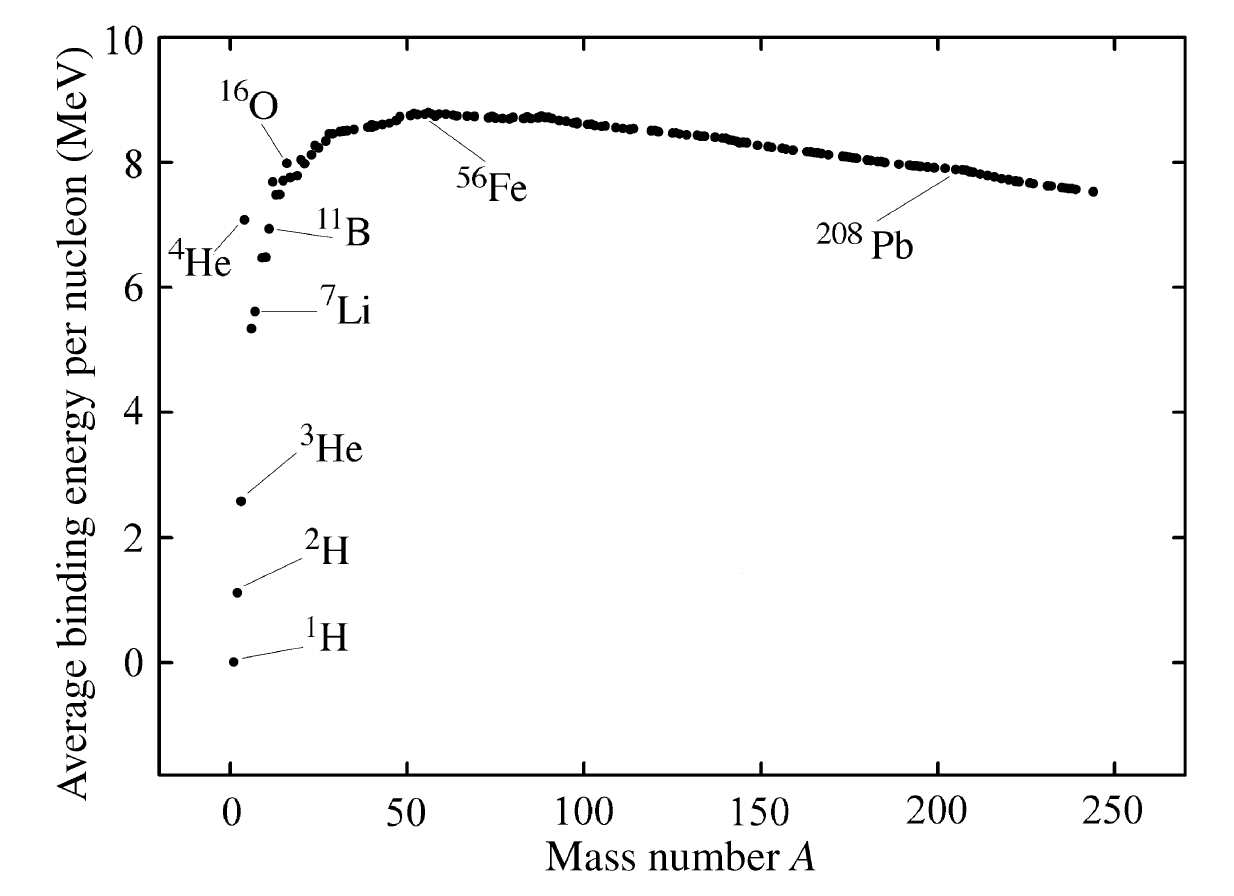
\includegraphics[width=0.8\linewidth]{figures/bindingenergy}
    \caption{Binding energies for nuclei that are stable or long-lived \cite{Hooshyar}.}
    \label{fig:bindingenergy}
\end{figure}
If we look at the distribution of stable nuclei (see figure~\ref{fig:nuclidmap}) we notice
that stable nuclei only occur in a very narrow band, other nuclei are unstable and decay sponatneously.
The decay is characerized by a \textit{decay constant} $\lambda$, which is related to the activity $\mathcal{A}$
by 
\begin{equation}\label{eq:decay}
    \mathcal{A} = -\frac{\partial N}{\partial t} = \lambda N 
\end{equation}
Where the activity $\mathcal{A}$ is typically given in Bequerel: $1 \textrm{Bq}= \textrm{decay}\cdot s^{-1}$ 
The solution to the differential equation in \eqref{eq:decay} yields:
\begin{equation}
    \mathcal{A}(t) = \lambda N_0 \exp(-\lambda t)
\end{equation}
with the initial condition $N_0 := N(t=t_0)$. 
The probability of an Atom to decay after time $t$ is thus:
\begin{equation}
    \mathcal{P}(t) = \int_{0}^{t}\lambda \exp(-\lambda t')\mathrm{d}t' = 1 -  \exp(-\lambda t)  \quad
    \textrm{with} \quad \int_{0}^{\infty}\lambda \exp(-\lambda t')\mathrm{d}t' = 1
\end{equation}
such that the probability density is $f(t) = \lambda \exp(-\lambda t)$.
Hence we can calculate the expectation value of a random variable $t$ within the probability space
$\Omega$ with the measure  $\mathcal{P}$:
\begin{equation}
    \tau := E[t] = \int_{0}^{\infty} t \lambda \exp(-\lambda t) \mathrm{d}t 
    =\lim_{t \rightarrow \infty}\left[ \frac{exp(-\lambda t) (1-\lambda t) - 1 }{\lambda} \right] 
= \frac{1}{\lambda}
\end{equation}
The half-life $t_{1/2}$ is obviously connected by $t_{1/2}= -\mathrm{log}(2)/ \lambda = - \tau \mathrm{log}(2)$.
\begin{figure}[htpb]
    \centering
    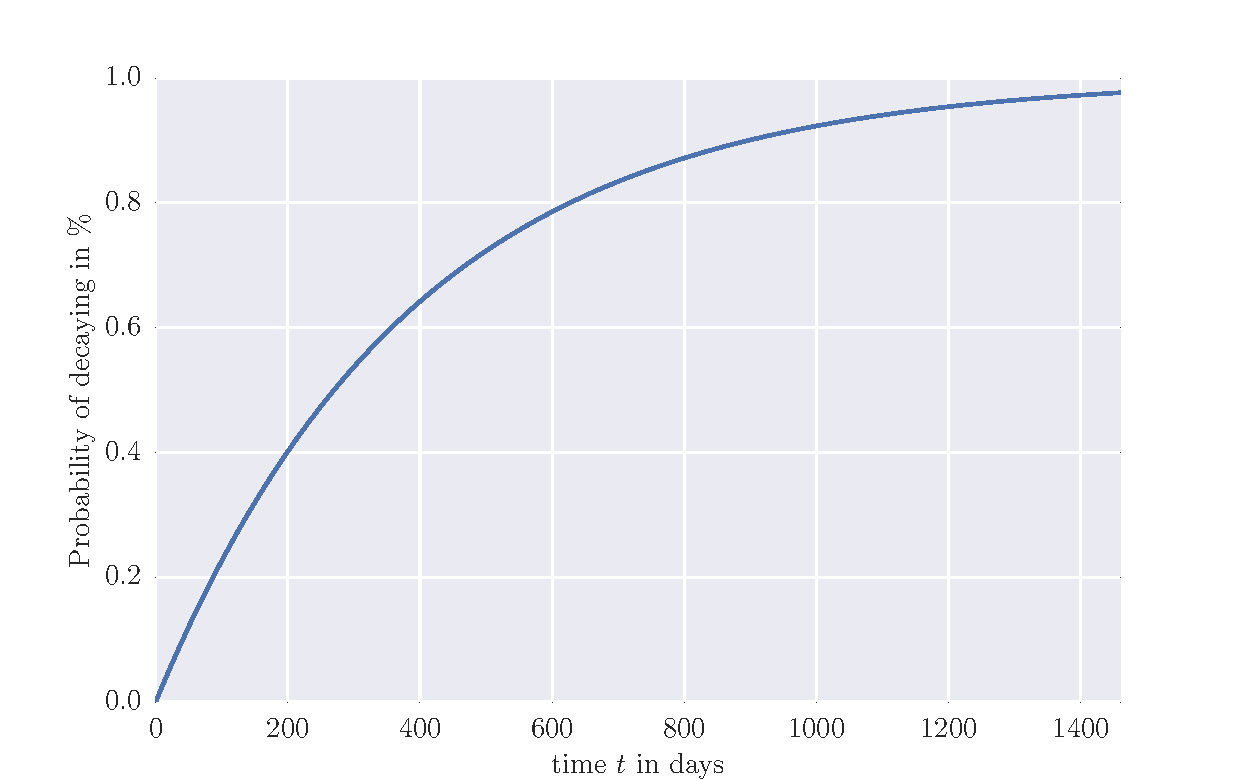
\includegraphics[width=0.9\linewidth]{analysis/figures/halflife}
    \caption{Probability $\mathcal{P}(t) = 1 -  \exp(-\lambda t)$ of an atom to decay after time $t$.
        Here we chose as an example the decay of
        $^{57}\textrm{Cs}\rightarrow ^{57}\textrm{Fe}$ with $t_{1/2}=270$ over a timerange
    of 4 years.}
    \label{fig:decay}
\end{figure}
\clearpage
\subsubsection{Semi-Empirical Mass Formula: The Liquid Drop Model}
\begin{figure}[htpb]
    \centering
    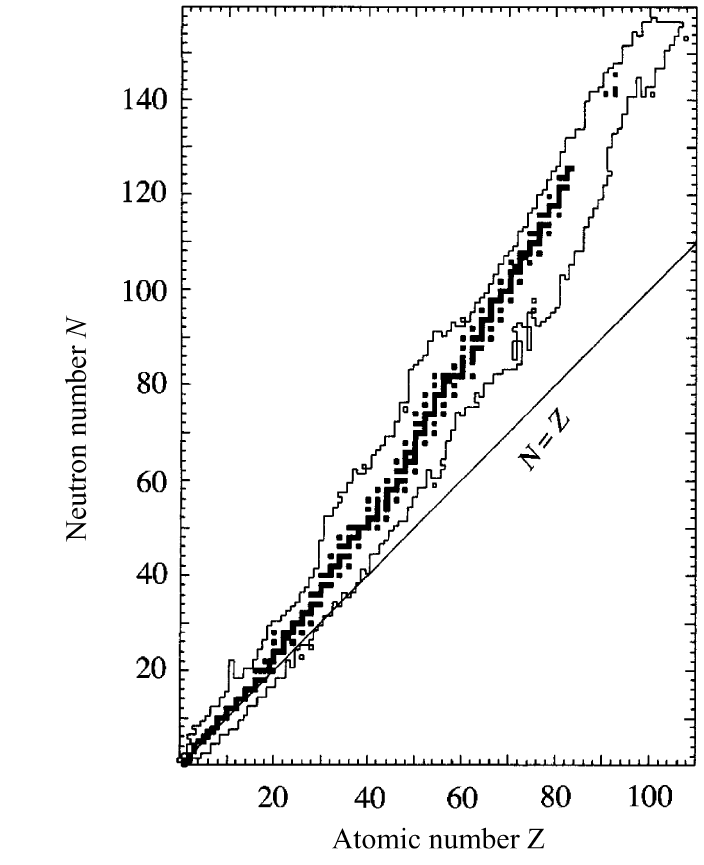
\includegraphics[width=0.6\linewidth]{figures/nuclidmap}
    \caption{Nuclid map of stable nuclei \cite{Hooshyar}: The squares are the long-lived nuclei
    occuing in nature; otherknown nuclei lie within the jagged lines and are unstable.}
    \label{fig:nuclidmap}
\end{figure}
\label{ssub:Semi-Empirical Mass Formula: The Liquid Drop Model}
We continue following \cite{Hooshyar}. We now approach an theoretic model which contains constants which
have to be fitted with experiments, thats why its called semi-empirical. 
The model was first established by Weizsäcker and will yield a 
good approximation for the atomic masses. The model is built upon the following assumptions, which turn
out to be valid in the regime we are looking at:
\begin{enumerate}
    \item The interior mass densities are approximately equal,
    \item their total binding energies are approximately proportional to their masses.
\end{enumerate}
This shows why the model is called ``Liquid Drop Model'', since (1.) relates to the equality of densities
of drops and (2) to the proportionality of latent heats of vaporization to the masses of a drops. 
Now we build up our energy in units of masses with different contributions:
\begin{equation}
    M_{tot} = \sum_{i=0}^{5} f_i 
\end{equation}
\begin{itemize}
    \item \textbf{Mass term:} 
First we take into account the atomic masses 
consisting of the mass of the nucleons and electrons:
\begin{equation}
    f_0 = Z(M_p + m_e) + (A-Z)M_n
\end{equation}
    \item \textbf{Volume term:} This term will estimate the effect of strong 
        nuclear forces proportional to the volume:
        \begin{equation}
            f_1 = -a_1 A
        \end{equation}
where $a_1$ has to be found depending on the volume. 
    \item \textbf{Surface term:} Since the volume does not take into account that nuclei at the surface are not
        interacting with as many nuclei than in the center, this term corrects the Volume energy by 
        the surface:
        \begin{equation}
            f_2 = a_2 A^{\frac{2}{3}}
        \end{equation}
        where we have assumed that the surface area leads to a decrease of binding energy, which would
        correspond to the surface tension energy in the classical liquid drop model.
    \item \textbf{Coulomb term:} The protons of each nucleus repell each other dependent on their number.
        If we assume a uniform charge distribution of radius proportional to $A^{\frac{1}{3}}$:
        \begin{equation}
            f_3 = a_3 \frac{Z(Z-1)}{A^{\frac{1}{3}}} \approx a_3 \frac{Z^2}{A^{\frac{1}{3}}} 
            \quad \text{(when we assume} \quad Z \gg 1)
        \end{equation}
    \item \textbf{Assymetric term:} Due to the Pauli principle the nuclei tend to broaden their distribution
        on energies, with leads to a positive energy correction:
\begin{equation}
    f_4 = a_4 \frac{(Z- \frac{A}{2})^2}{A}
\end{equation}
    \item \textbf{Pairing term:} This correction accounts for the tendency of proton pairs and neutron pairs
        to occur, where an even number of particles is more stable than an odd number:
      \begin{align}
          \begin{split}
          \label{eq:pair}
          f_5 &= -f(A) \quad \text{if $Z$ even and $A-Z=N$ even}\\
          f_5 &=  0    \quad \text{if $Z$ even but $A-Z=N$ odd or $Z$ odd but $A-Z=N$ even}\\
          f_5 &=  f(A) \quad \text{if $Z$ odd and $A-Z=N$ odd}
          \end{split}
      \end{align}
      Where the function $f(A)$ should be estimated by fitting the data, 
      often $f(A) = a_5 A^{-\frac{1}{2}}$ is used.
\end{itemize}
\subsubsection{Unstable States}
\label{ssub:Unstable States}
If we want investigate the form of the energy distribution of a decay, we have to 
introduce the \textit{natural decay width}, given by
\begin{equation}
    \Gamma_f = \frac{\hbar}{\tau_f} 
\end{equation}
which can be defined for each channel $f$, such that in total we get
\begin{equation}
    \Gamma = \sum_{f} \Gamma_f
\end{equation}
Where we can define the \textit{branching ratio} for channel $f$ as:
\begin{equation}
    B_f = \frac{\Gamma_f}{\Gamma}
\end{equation}
The energy distribution of the unstable state to a final state $f$ resolves into a 
\textit{Breit-Wigner-distribution}:
\begin{equation}
    N_f(M_f) = \frac{\Gamma_f}{(M_f-M_i)^2 c^4 + \Gamma^2/4}
\end{equation}
With the mass of the decaying state $M_i$ and the invariant mass of decay products $M_f$.
\begin{figure}[htpb]
    \centering
    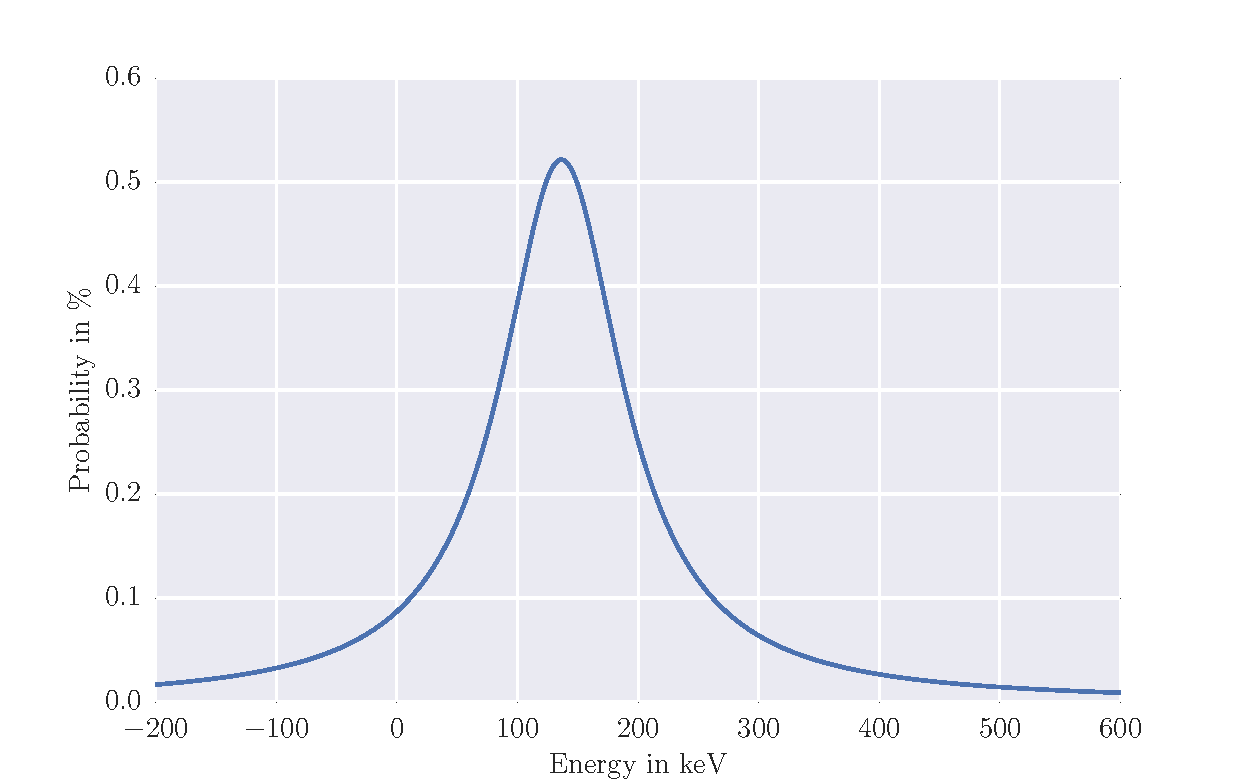
\includegraphics[width=0.9\linewidth]{analysis/figures/breit_wigner}
    \caption{Breit-Wigner distribution. Here again with
        $^{57}Cs\rightarrow ^{57}Fe$ with $t_{1/2}=270$. Hence we have $M_i = 136.5$keV and
    $\Gamma_f = \hbar / \textrm{log}(2)t_{1/2} = 122$keV, which resamples in the width of the curve.}
    \label{fig:name}
\end{figure}
\clearpage


